\begin{frame}{Autour du monde}
  \footnotesize
  En groupes de 4, chosissez l'un des pays ou régions au-dessous, lisez l'article lié à ce pays ou cette région et préparez un bref résumé \gloss{short summary} de l'article à présenter à la classe.
  \begin{columns}
    \column{0.45\textwidth}
      \begin{enumerate}
        \item Haïti
          \item[] \href{https://tinyurl.com/nxpzpxce}{https://tinyurl.com/nxpzpxce}
        \item Sénégal
          \item[] \href{https://tinyurl.com/59bns5vn}{https://tinyurl.com/59bns5vn}
        \item Martinique
          \item[] \href{https://tinyurl.com/2euua8wm}{https://tinyurl.com/2euua8wm}
        \item Canada
          \item[] \href{https://tinyurl.com/mrznnbxb}{https://tinyurl.com/mrznnbxb}
        \item Algérie
          \item[] \href{https://tinyurl.com/3juy8uuv}{https://tinyurl.com/3juy8uuv}
      \end{enumerate}
    \column{0.55\textwidth}
      \only<1>{
        \begin{center}
          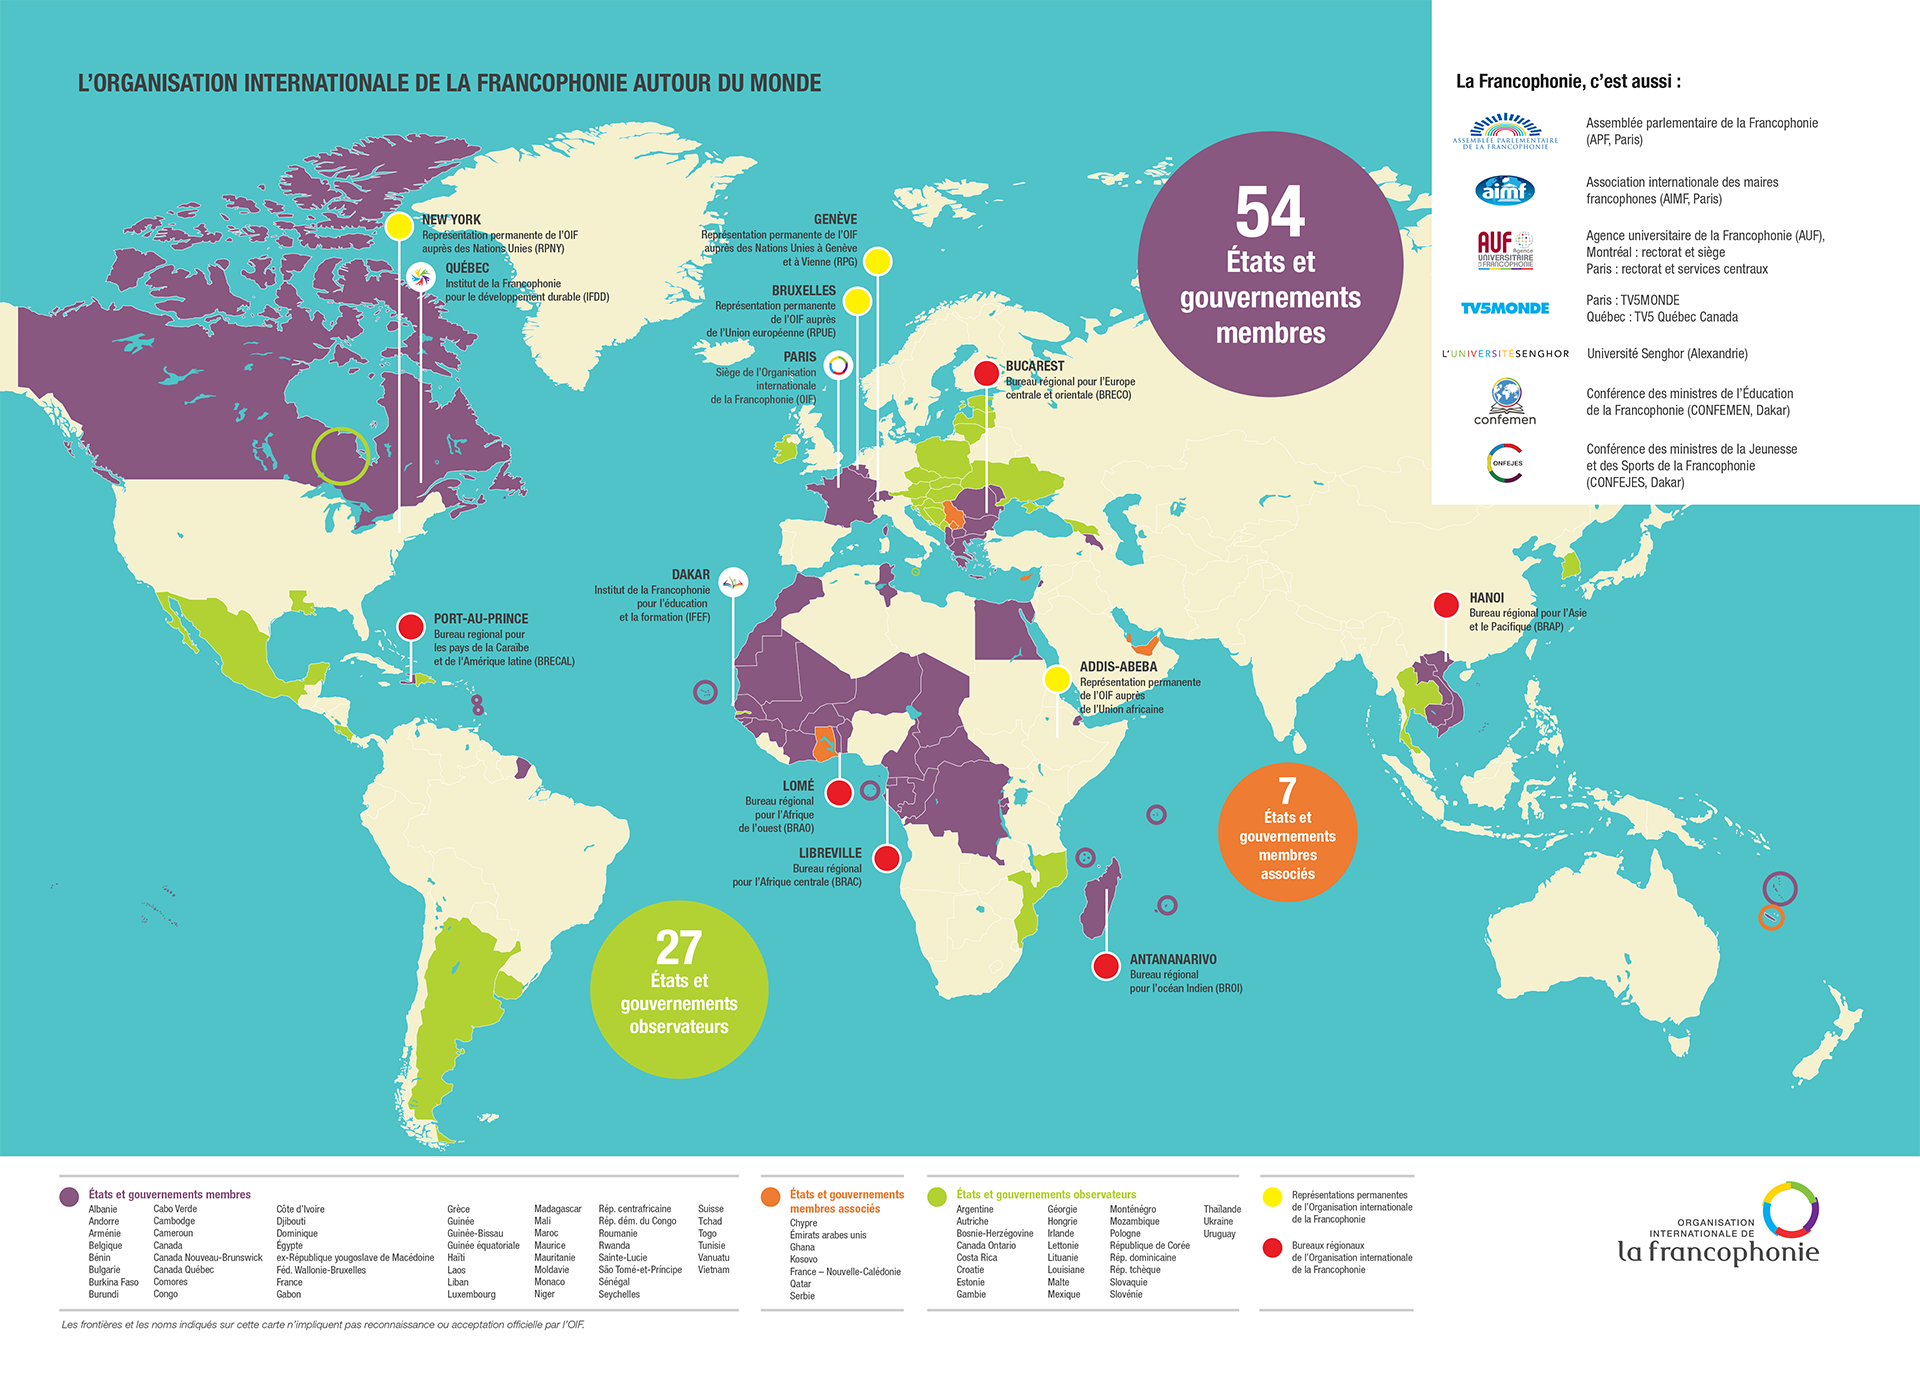
\includegraphics[scale=0.09]{francophonie.png}
        \end{center}
      }
      \only<2->{
        Pendant que vous écoutez, écrivez au moins une question pour les présentateurs.
      }
  \end{columns}
\end{frame}